%\documentclass[a4paper,12pt]{article}

%\usepackage{graphics}
%\usepackage[pdftex]{graphicx}

%\begin{document}

\subsection{Topologie de l'Internet}
\subparagraph{}
Comme expliqu\'e pr\'ec\'edemment, Internet n'est pas un seul grand r\'eseau. Il s'agit en fait de l'interconnexion de plusieurs r\'eseaux ou syst\`emes autonomes (AS). Un syst\`eme autonome est un r\'eseau r\'egi par une m\^eme administration et soumis \`a un ensemble de r\`egles de routage internes consistantes. Les AS sont reli\'es entre eux par des liaisons physiques; celles-ci sont associ\'ees \`a des contrats \'economiques d'interconnexion. Ils sont la plupart du temps un des deux contrats suivants:
\begin{description}
 \item[PEER : ] accord commercial \`a travers lequel les clients respectifs de deux AS peuvent communiquer entre eux sans que les AS ne doivent se payer la connexion,
 \item[Transit : ] il s'agit d'un lien commercial \`a travers lequel un AS est le client d'un autre afin d'y transmettre tout ou partie de son trafic. On notera C2P pour un arc du client vers le fournisseur et P2C pour les arcs dans le sens oppos\'e.
\end{description}
\par
Au coeur de l'Internet, on trouve les op\'erateurs appel\'es \textit{Tier One} qui sont en th\'eorie reli\'es deux \`a deux par des liens de type PEER au sein d'une structure tr\`es maill\'ee, presque un \textit{full-mesh} aussi appel\'e \textit{clique} en th\'eorie des graphes. Les \textit{Tier One} sont les grands op\'erateurs qui forment le coeur de l'Internet.
\par
%Ils sont tous reli\'es deux \`a deux par des accords de type PEER, et ne peuvent pas se d\'econnecter. Meule nous a expliqué le contraire... Avec ses exemple sur Sprint, de plus tu l'a déjà dit pour la partie connexion en PEER
 Les \textit{Tier One} peuvent atteindre n'importe quelle destination sur Internet sans avoir \`a payer une seule connexion, puisqu'\`a plus ou moins haut niveau, tout AS est client potentiel d'un \textit{Tier One}. On retrouve parmis les \textit{Tier One} quelques grands noms des télécommunications (qui ne sont pas forcément des fournisseurs d'acc\`es) : Orange, Verizon Business, Sprint, AT\&T...
\par
Sont reli\'es \`a ces grands op\'erateurs d'autres AS qui peuvent eux-m\^eme \^etre reli\'es \`a d'autres et ainsi de suite. En outre, de fa\c con locale, on peut retrouver des structure en full-mesh.
\par
Globalement, Internet (IPv4) a une structure connexe, c'est-\`a-dire que si l'on prend deux AS au hasard, il existe au moins un chemin qui les relie. Il revient donc \`a chaque AS d'assurer la visibilit\'e de ses clients \`a travers le r\'eseau.
\par
En bout de cha\^ine, il y a les AS dits stubs. Ce sont des AS qui sont clients d'un ou plusieurs autres AS mais qui n'ont pas de client. Quand un AS stub est reli\'e \`a un seul AS, on dit qu'il est \textit{monohom\'e}. Si, au contraire, il est le client de plusieurs autres AS en m\^eme temps, on dit qu'il est \textit{multi-hom\'e}. Le multi-homing permet de palier à la défaillance de l'un de ses fournisseurs d'accès.
\par
La topologie d'internet est hierarchique. C'est une sorte de pyramide avec à son sommet le \textit{Tier One} et à sa base les stubs.

\subsubsection{Repr\'esentation d'Internet}
\subparagraph{}
De fa\c con pratique, on peut repr\'esenter Internet comme un graphe o\`u les sommets sont les AS et les ar\^etes les liens entre les AS. La figure \ref{topologie} montre un exemple de cette repr\'esentation avec un coeur de l'Internet compos\'e de trois AS auxquels sont connect\'es d'autres AS.
\par
En raison du grand nombre d'AS, il est tr\`es difficile de repr\'esenter de fa\c con synth\'etique l'ensemble du r\'eseau. Les relations C2P et P2C peuvent \^etre vues comme port\'ees des arcs verticaux et les relations de peering peuvent \^etre consid\'er\'ees comme des relations horizontales.
%On remarque que certain AS peuvent \^etre client aupr\`es de plusieurs AS en m\^eme temps. Cette m\'ethode est utile pour garantir un connectivit\'e m\^eme en cas de d\'efaillance d'une connection. Tu te répètes avec ce qu'il y au-dessus

\begin{figure}[H]
\centering
 \fbox
 {
 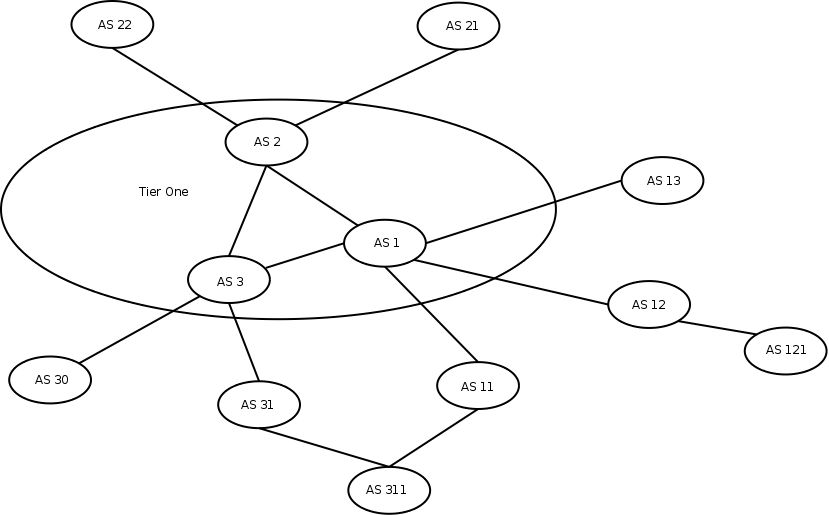
\includegraphics[width=16cm]{./schema/topologie_internet.png}
 }
  \caption{\label{topologie}Topologie d'Internet, exemple de repr\'esentation}
\end{figure}



%\end{document}
